\documentclass[14pt, a4paper]{extarticle}
\usepackage{mospolytech_coursework}
\usepackage{listings}
\usepackage{xcolor}
% \usepackage{xurl}
% \usepackage{url}

\lstset{
    language=Python,
    basicstyle=\ttfamily\small,
    keywordstyle=\color{blue},
    stringstyle=\color{red},
    commentstyle=\color{green!50!black},
    breaklines=true,
    breakatwhitespace=true,
    breakautoindent=true,
    postbreak=\space,
    numbers=left,
    numberstyle=\tiny\color{gray},
    stepnumber=1,
    numbersep=5pt,
    frame=single,
    tabsize=4,
    showstringspaces=false
}

% Определение данных
\newcommand{\theme}{%
    Разработка веб-приложения для ведения семейного бюджета%
    }
\newcommand{\subject}{Разработка веб-приложений}
\newcommand{\student}{Момина Антонина Алексеевна}
\newcommand{\group}{241-327}
\newcommand{\teacher}{Кружалов Алексей Сергеевич}

\begin{document}

% Титульный лист
\include{title}

% Задание
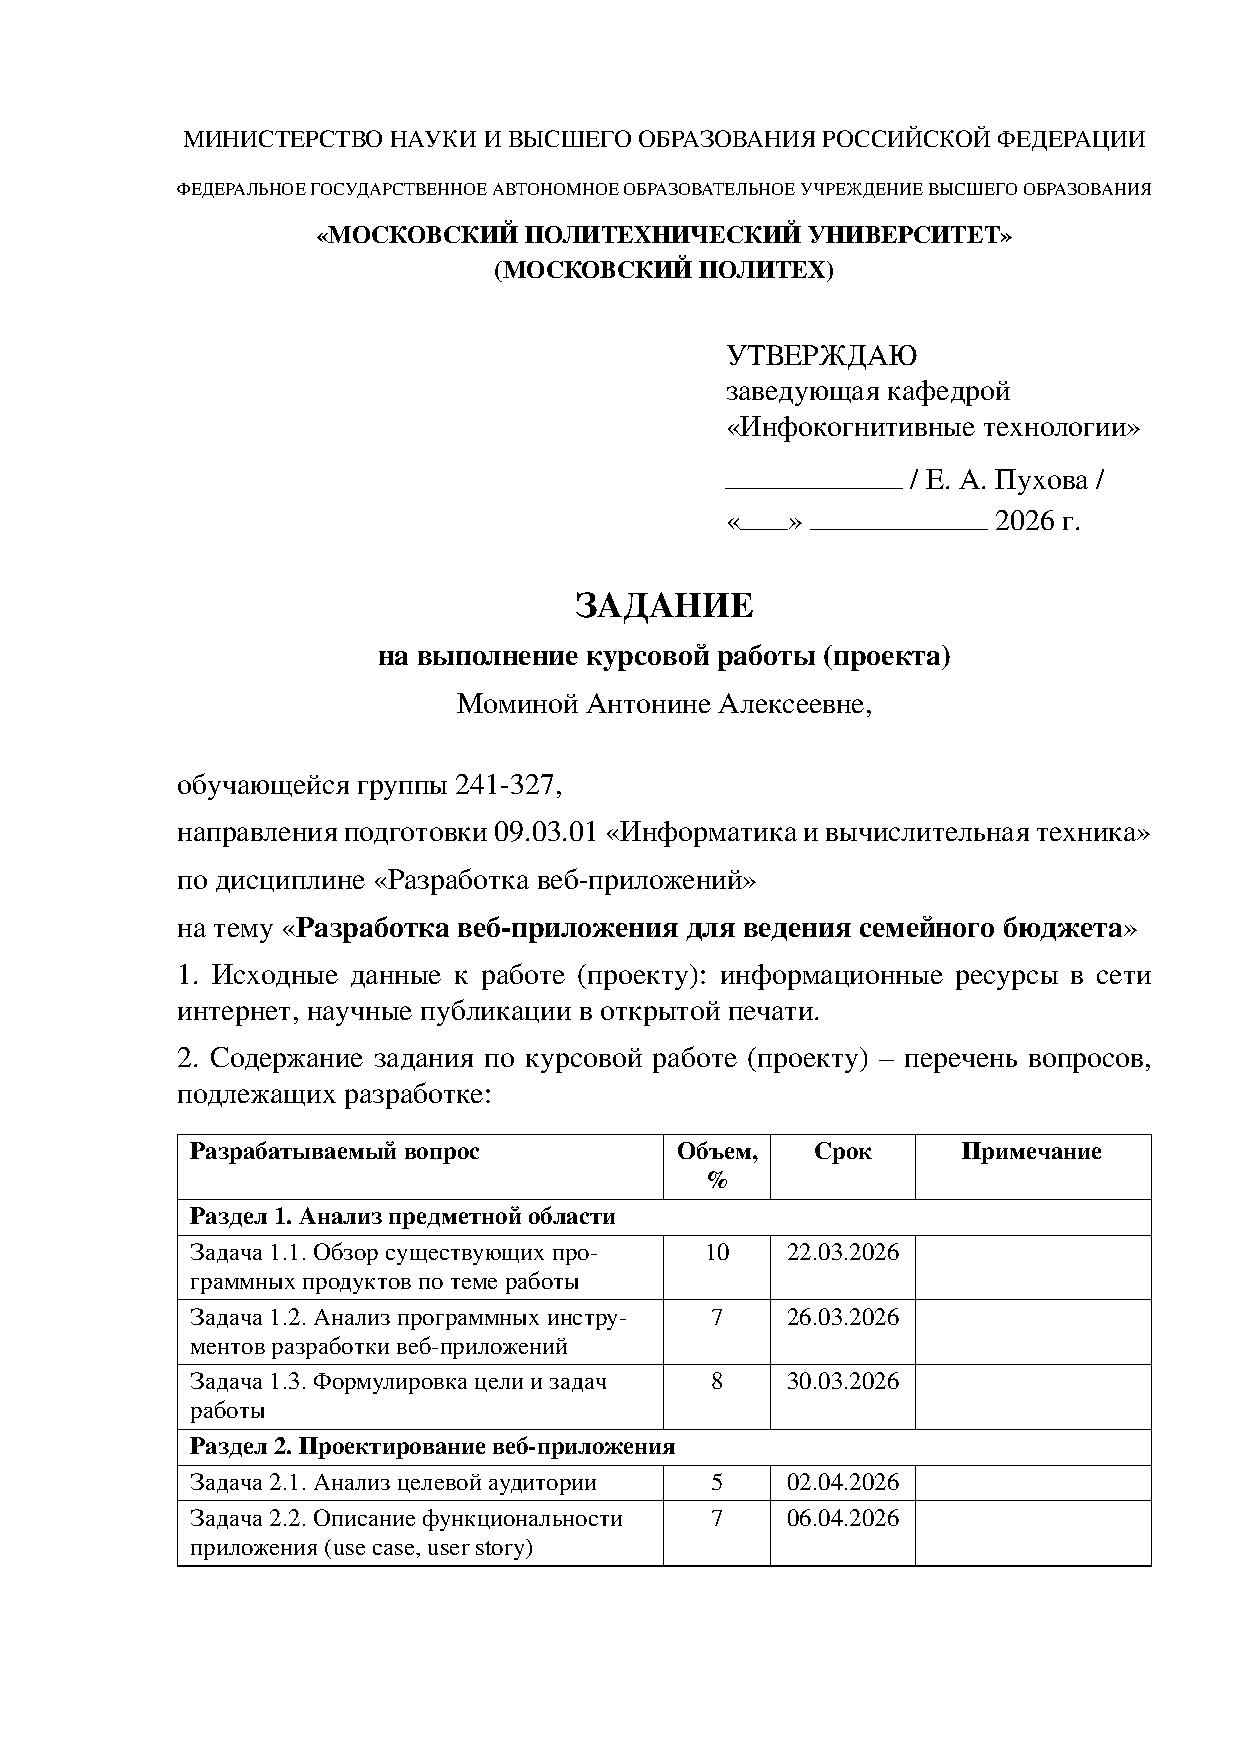
\includepdf[pages=-]{task.pdf}

% Содержание
\tableofcontents

% Введение
\section*{Введение}
\addcontentsline{toc}{section}{Введение}

В современных условиях эффективное управление личными и семейными финансами является важной задачей для большинства людей. Однако многие семьи сталкиваются с трудностями при контроле доходов и расходов.

\textbf{Проблема.} Основная проблема состоит в том, что у людей часто нет удобного и надёжного инструмента для систематического учёта финансов. Многие ведут записи в заметках или простых таблицах Excel. Это приводит к неконтролируемым тратам, невозможности правильно спланировать бюджет и снижению финансовой стабильности. Кроме того, существующие приложения часто неудобны для совместного использования несколькими людьми, имеют ограниченные возможности аналитики и не всегда позволяют работать с чеками и документами.

\textbf{Актуальность.} Тема учёта семейных финансов остаётся актуальной в 2026 году. Согласно исследованию Аналитического центра НАФИ и страховой компании «Росгосстрах Жизнь» (2025)~\cite{nafi2025}, индекс финансовой грамотности россиян снизился до 12,61 балла из 21 возможного. Доля граждан с низким уровнем финансовой грамотности выросла до 34~\%, а среди молодёжи 18--34 лет составляет 51~\%. Почти половина работающих россиян регулярно испытывает финансовые трудности.

В условиях прогнозируемой инфляции 4,5--5,5~\% (по данным Банка России на 2026 год)~\cite{cbr2026} семьи всё больше нуждаются в удобном инструменте для ведения общего семейного бюджета, отслеживания расходов всех членов семьи, загрузки чеков и получения наглядной статистики.

\textbf{Степень разработанности проблемы.} На сегодняшний день существует множество приложений для учёта финансов. Они позволяют вести учёт транзакций, ставить бюджеты и смотреть простые отчёты. Однако большинство из них имеют существенные недостатки: платные премиум-функции, слабая поддержка совместной работы нескольких пользователей, ограниченные возможности загрузки файлов и не всегда удобная аналитика. Готовых открытых веб-решений, которые одновременно включают систему ролей пользователей, полноценный CRUD-интерфейс, загрузку и выгрузку файлов чеков и глубокую агрегацию данных, относительно немного. Это определяет место и актуальность настоящей курсовой работы.

\textbf{Объект исследования} — процесс учёта и анализа доходов и расходов семейного бюджета с помощью веб-технологий.

\textbf{Предмет исследования} — методы и средства разработки веб-приложения для управления личными финансами, включающего аутентификацию, авторизацию по ролям, CRUD-операции, агрегацию данных и работу с файлами.

\textbf{Цель работы} — разработать веб-приложение для учёта расходов и доходов семейного бюджета, которое обеспечит удобный совместный контроль финансов, аналитику и безопасность данных.

Для достижения поставленной цели необходимо решить следующие \textbf{задачи}:

\begin{itemize}
    \item проанализировать существующие программные продукты и технологии разработки веб-приложений для управления финансами;
    \item определить требования целевой аудитории и спроектировать функциональность приложения (диаграммы вариантов использования, User Story);
    \item разработать модель данных (ER-диаграмму, логическую и физическую схемы базы данных);
    \item спроектировать пользовательский интерфейс (wireframes);
    \item реализовать систему аутентификации и авторизации с проверкой прав доступа по ролям;
    \item разработать CRUD-интерфейс для основных сущностей (транзакции, категории, бюджеты);
    \item реализовать механизмы загрузки и выгрузки файлов (чеки, отчёты) и агрегацию данных с визуализацией статистики;
    \item провести тестирование, деплой приложения и оформить отчётную документацию.
\end{itemize}

\textbf{Актуальность темы.} В работе применялись методы системного анализа, сравнительный анализ существующих решений, структурное и объектно-ориентированное проектирование. Для реализации использовались современные веб-технологии (backend, frontend и база данных). Визуализация данных выполнялась с помощью специализированных библиотек. Тестирование проводилось по функциональным и нефункциональным требованиям.

Структура отчёта соответствует логике поставленных задач и включает анализ предметной области, проектирование, описание реализации и заключение.


% Основная часть
\section*{Глава 1. Анализ предметной области}
\addcontentsline{toc}{section}{Глава 1. Анализ предметной области}
\stepcounter{section}

\subsection{Обзор существующих программных продуктов}

На рынке представлено большое количество приложений для учёта личных и семейных расходов. Большинство из них — это мобильные приложения (Android/iOS). Полноценных веб-приложений, специально ориентированных на совместный семейный бюджет, на 2026 год очень мало.

Для сравнения были выбраны наиболее популярные решения: Дзен-мани, CoinKeeper, Monefy и Money Lover. В таблице ниже приведены их ключевые характеристики с точки зрения семейного использования.

\begin{table}[h]
	\centering
	\caption{Сравнение популярных приложений для учёта финансов}
	\label{tab:competitors}
	
	{\fontsize{12}{14}\selectfont
	\setlength{\tabcolsep}{6pt}
	
	\begin{tabular}{|p{3.7cm}|p{3.7cm}|p{3.5cm}|p{3.5cm}|}
	\hline
	\textbf{Характеристика} 
		& \textbf{Дзен-мани} 
		& \textbf{Monefy} 
		& \textbf{Money Lover} \\
	\hline
	
	Платформа 
		& Мобильное 
		& Мобильное 
		& Мобильное + Web \\
	\hline
	
	Совместный бюджет 
		& Полноценный 
		& Сильно ограничен 
		& Есть (в Premium) \\
	\hline
	
	Загрузка чеков 
		& Есть (QR-сканирование) 
		& Ограничено 
		& Есть (фото) \\
	\hline
	
	Веб-версия 
		& Ограниченная 
		& Отсутствует 
		& Полноценная \\
	\hline
	
	Стоимость ключевых функций 
		& Премиум-подписка (многие отчёты и прогнозы) 
		& Премиум для расширенной аналитики и синхронизации 
		& Unlimited wallets и shared budgets — только Premium \\
	\hline
	\end{tabular}
	
	}
	\end{table}


Как видно из таблицы, у каждого рассмотренного приложения есть существенные недостатки именно при семейном использовании:

\begin{itemize}
    \item \textbf{Дзен-мани} — лучший функционал совместного бюджета, но большинство важных отчётов, прогнозов и расширенной аналитики доступны только по платной подписке.
    \item \textbf{Monefy} — очень простой и интуитивный интерфейс, но совместный доступ сильно ограничен, а полноценной веб-версии нет.
    \item \textbf{Money Lover} — имеет веб-версию, однако создание нескольких общих кошельков и расширенные возможности бюджетирования также требуют платной подписки.
\end{itemize}

Таким образом, несмотря на обилие мобильных решений, на рынке практически отсутствует удобное, бесплатное (или полностью функциональное в базовой версии) веб-приложение, которое одновременно предоставляет:

\begin{itemize}
    \item полноценную совместную работу нескольких пользователей,
    \item систему ролей и разграничения прав доступа,
    \item удобную загрузку и выгрузку файлов (чеков, отчётов),
    \item глубокую агрегацию данных и наглядную статистику,
    \item доступ с любого устройства без установки приложений.
\end{itemize}

\textbf{Вывод.} Разработка собственного веб-приложения для учёта семейных расходов позволит устранить указанные недостатки существующих решений и создать удобный, бесплатный в базовой функциональности инструмент, специально ориентированный на совместное использование всей семьёй.


\subsection{Анализ программных инструментов разработки}

Для реализации веб-приложения были рассмотрены популярные технологии и стеки разработки. Особое внимание уделялось простоте освоения, скорости разработки, наличию необходимого функционала (аутентификация, работа с базой данных, загрузка файлов, визуализация) и подходящему уровню сложности для курсового проекта.

% \textbf{Анализ backend-фреймворков}

Наиболее распространёнными Python-фреймворками для создания веб-приложений в 2026 году являются Django, Flask и FastAPI.

\textbf{Django} — мощный full-stack фреймворк, включающий в себя большое количество готовых компонентов («батарейки из коробки»): встроенную систему аутентификации, ORM, админ-панель и механизмы защиты. Главное преимущество — высокая скорость разработки и хорошая безопасность. Основной недостаток — избыточная сложность и «тяжеловесность» для небольшого учебного проекта.

\textbf{FastAPI} — современный высокопроизводительный асинхронный фреймворк для создания API. Отличается отличной поддержкой типизации и автоматической генерацией документации. Преимущества: высокая скорость работы. Недостатки: избыточен для классического CRUD-приложения с серверным рендерингом шаблонов.

\textbf{Flask} — лёгкий микрофреймворк, который предоставляет только базовый функционал. Все необходимые расширения подключаются по мере необходимости. Главные преимущества — высокая гибкость, минимализм, простота изучения и отличная читаемость кода.

% \textbf{Анализ систем управления базами данных}

Для управления базой данных рассматривались две основные СУБД: SQLite и PostgreSQL.

\textbf{SQLite} — простая файловая база данных, не требующая установки сервера. Преимущества: крайне простая настройка, нулевые затраты на развертывание, высокая скорость для небольших проектов. Недостатки: слабая поддержка нескольких пользователей одновременно, ограниченные возможности по масштабированию и ограниченный функционал.

\textbf{PostgreSQL} — полноценная клиент-серверная реляционная СУБД. Преимущества: высокая производительность при работе с несколькими пользователями, возможности сложных запросов, хорошая масштабируемость и надёжность. Недостатки: более сложная настройка по сравнению с SQLite.

% \textbf{Анализ frontend-технологий}

Для создания пользовательского интерфейса сравнивались Bootstrap 5 и полноценные JavaScript-фреймворки React и Vue.

\textbf{Bootstrap 5} — CSS-фреймворк с готовыми компонентами и встроенной адаптивностью. Преимущества: очень быстрая вёрстка, минимальный порог вхождения, удобен для адаптивности. Недостатки: менее гибкий при создании сложной интерактивной логики.

\textbf{React} и \textbf{Vue} — мощные JavaScript-фреймворки для создания веб-приложений. Преимущества: высокая интерактивность, компонентный подход, отличная производительность при большом объёме данных. Недостатки: значительно более сложные в использовании, необходимость в дополнительных инструментах (Vite, Redux/Vuex и т.д.), что избыточно для курсового проекта.


После проведённого анализа был выбран следующий стек разработки:

\begin{itemize}
    \item \textbf{Backend}: Python 3.12 + Flask 3.1
    \item \textbf{ORM}: Flask-SQLAlchemy
    \item \textbf{Аутентификация и авторизация}: Flask-Login + Flask-Bcrypt
    \item \textbf{База данных}: PostgreSQL
    \item \textbf{Frontend}: HTML5, CSS3, JavaScript, Bootstrap 5.3
    \item \textbf{Визуализация данных}: Chart.js
    \item \textbf{Дополнительные инструменты}: Git, Visual Studio Code
\end{itemize}

Данный стек обеспечивает оптимальный баланс между простотой реализации, читаемостью кода и требуемым функционалом. Flask позволяет глубоко понять принципы построения веб-приложений без избыточных абстракций, что особенно важно в рамках курсовой работы. PostgreSQL выбрана с целью приближения проекта к реальным условиям разработки.



\subsection{Формулировка цели и задач работы}

\textbf{Цель работы} — разработать веб-приложение для учёта расходов и доходов семейного бюджета, обеспечивающее удобный совместный контроль финансов, прозрачность трат и наглядную аналитику для всех членов семьи.

Для достижения поставленной цели необходимо решить следующие задачи:

\begin{enumerate}
    \item Проанализировать существующие программные продукты и технологии разработки веб-приложений для управления семейными финансами.
    \item Определить требования целевой аудитории и спроектировать функциональность приложения (диаграммы вариантов использования, User Story).
    \item Разработать модель данных (ER-диаграмму, логическую и физическую схемы базы данных).
    \item Создать макеты пользовательского интерфейса (wireframes).
    \item Реализовать систему аутентификации и авторизации пользователей с разделением прав доступа по ролям.
    \item Разработать CRUD-интерфейс для основных сущностей (транзакции, категории, бюджеты).
    \item Реализовать механизмы загрузки и выгрузки файлов (чеки, отчёты) и систему агрегации данных с визуализацией статистики.
    \item Провести тестирование приложения, выполнить деплой и оформить отчётную документацию.
\end{enumerate}

В результате работы будет создано полноценное веб-приложение, соответствующее всем требованиям курсового проекта.

\section*{Глава 2. Проектирование веб-приложения}
\addcontentsline{toc}{section}{Глава 2. Проектирование веб-приложения}
\stepcounter{section}


\subsection{Анализ целевой аудитории}

Для успешной разработки веб-приложения по ведению семейного бюджета необходимо чётко понимать, для кого оно создаётся, какие задачи будут решать пользователи и с какими ограничениями (техническими, финансовыми, временными) они сталкиваются в повседневной жизни.

На основе потребностей, технической подготовки и мотивации к ведению учёта была выделена одна, самая многочисленная и проблемная категории пользователей: семьи с совместным (полностью или частично) бюджетом.

\subsubsection{Проблематика}

Семьи с совместным бюджетом сталкиваются с рядом типичных проблем:
\begin{itemize}
    \item Отсутствие финансовой прозрачности. Часто только один из партнёров имеет полное представление о доходах и расходах, что порождает недоверие.
    \item Споры о тратах и невозможность объективной оценки. При отсутствии единой записной книжки невозможно объективно сравнить расходы разных членов семьи.
    \item Сложность планирования крупных покупок. При обдумывании больших трат необходимо иметь актуальную картину по доходам и обязательным расходам.
    \item Необходимость контролировать разные типы расходов. Семейный бюджет неоднороден: есть общие траты и личные траты. Без разграничения можно незаметить лишние расходы.
    \item Разная мотивация к ведению учёта. Один партнёр может хотеть детальной аналитики, а второй лишь изредка вносить расходы. Инструмент должен учитывать оба типа поведения.
\end{itemize}

\subsubsection{Потребности ЦА}

На основе выявленных проблем были сформулированы следующие потребности, которые должно закрыть разрабатываемое приложение:

\begin{table}[h]
    \centering
    \caption{Потребности целевой аудитории}
    \label{tab:target-audience-needs}

    {\fontsize{12}{14}\selectfont
	\setlength{\tabcolsep}{6pt}

    \begin{tabular}{|p{4cm}|p{8cm}|p{3cm}|}
        \hline
        \textbf{Потребность} & \textbf{Описание} & \textbf{Задача из ТЗ} \\
        \hline
        Единое хранилище & Все транзакции семьи в одном месте, доступ с любого устройства & 3.3 (CRUD) \\
        \hline
        Разделение по ролям & Администратор, родитель, ребенок & 3.2 (авторизация с ролями) \\
        \hline
        Категоризация трат & Общие и личные категории, возможность создания/редактирования & 3.3 (категории) \\
        \hline
        Агрегация по участникам & Автоматический подсчёт расходов каждого члена семьи за период & 3.5 (аналитика) \\
        \hline
        Базовые отчёты & По периодам, категориям, участникам & 3.5 (статистика) \\
        \hline
        Привязка чеков & Загрузка фото/скана чека к транзакции & 3.4 (файлы) \\
        \hline
        Наглядная визуализация & Диаграммы и графики для быстрого понимания структуры расходов & 3.5 (Chart.js) \\
        \hline

    \end{tabular}
    }
\end{table}

\subsubsection{Портрет типичного представителя категории}

\begin{itemize}
    \item Семейное положение: состоит в браке или зарегистрированном партнёрстве.
    \item Состав семьи: 2–4 человека (родители + 1–2 детей).
    \item Используемые устройства: смартфон, ноутбук или ПК.
\end{itemize}

\subsubsection{Ключевые функции приложения}

На основе анализа проблем и потребностей выделен основной набор функций:

\begin{table}[h]
    \centering
    \caption{Основные функции}
    \label{tab:main-functions}

    {\fontsize{12}{14}\selectfont
	\setlength{\tabcolsep}{6pt}

    \begin{tabular}{|p{8cm}|p{4cm}|p{3cm}|}
        \hline
        \textbf{Функция} & \textbf{Важность} & \textbf{Реализация} \\
        \hline
        Аутентификация и разделение ролей & Критическая & Задача 3.2 \\
        \hline
        CRUD для транзакций & Критическая & Задача 3.3 \\
        \hline
        Фильтрация по дате, категории, участнику & Высокая & Задача 3.3 \\
        \hline
        Управление категориями (CRUD) & Высокая & Задача 3.3 \\
        \hline
        Управление бюджетами/лимитами & Высокая & Задача 3.3 \\
        \hline
        Визуализация (диаграммы) & Высокая & Задача 3.5 \\
        \hline
        Загрузка чеков & Средняя & Задача 3.4 \\
        \hline
        Экспорт отчёта & Средняя & Задача 3.4 \\
        \hline

    \end{tabular}
    }
\end{table}

\subsection{Описание функциональности приложения}


\subsection{Проектирование модели данных}


\subsection{Разработка макетов страниц}


\section*{Глава 3. Разработка веб-приложения}
\addcontentsline{toc}{section}{Глава 3. Разработка веб-приложения}
\stepcounter{section}

В соответствии с результатами проектирования было разработано веб-приложение для ведения семейного бюджета.

\subsection{Вёрстка HTML страниц}

Разработка пользовательского интерфейса началась с создания базового шаблона \texttt{base.html}, который определяет общую структуру всех страниц приложения. Шаблон включает:
\begin{itemize}
    \item заголовок страницы с динамическим заголовком;
    \item подключение Bootstrap 5.3 (CSS и JS) через CDN;
    \item подключение кастомных стилей \texttt{style.css};
    \item навигационную панель (navbar), содержимое которой зависит от роли пользователя (owner, member, admin);
    \item блок для отображения flash-сообщений (уведомлений);
    \item основную область контента (блок \texttt{content});
    \item футер с копирайтом.
\end{itemize}

На основе базового шаблона были свёрстаны следующие страницы:
\begin{itemize}
    \item \texttt{auth/login.html} --- страница входа;
    \item \texttt{auth/register.html} --- страница регистрации (выбор роли: владелец/участник, поле email и кода семьи);
    \item \texttt{dashboard/owner\_dashboard.html} --- дашборд владельца семьи;
    \item \texttt{dashboard/member\_dashboard.html} --- дашборд участника семьи;
    \item \texttt{dashboard/admin\_dashboard.html} --- панель администратора;
    \item \texttt{dashboard/member\_stats.html} --- страница просмотра статистики участника (для владельца);
    \item \texttt{transactions.html} --- управление транзакциями с фильтрацией;
    \item \texttt{categories.html} --- управление категориями;
    \item \texttt{members.html} --- управление участниками семьи;
    \item \texttt{profile.html} --- страница профиля пользователя;
    \item \texttt{admin/all\_transactions.html} --- просмотр всех транзакций (админ);
    \item \texttt{admin/all\_files.html} --- просмотр всех загруженных файлов (админ).
\end{itemize}


\subsection{Реализация модуля авторизации}

Модуль авторизации реализован с использованием расширений \texttt{Flask-Login} (управление сессиями) и \texttt{bcrypt} (хэширование паролей) через методы \texttt{set\_password} и \texttt{check\_password} в модели \texttt{User}.

Регистрация пользователя реализована в маршруте \texttt{/auth/register} с учётом ролевой модели:
\begin{itemize}
    \item При выборе роли \textbf{«Владелец»} автоматически создаётся новая семья с названием «Семья \{username\}» и генерируется 6-значный код-приглашение (формата FAM-XXXXXX). Пользователь становится владельцем семьи. Также автоматически создаются 8 категорий по умолчанию: Продукты, Транспорт, Коммунальные услуги, Зарплата, Подработка, Кафе и рестораны, Развлечения, Одежда.
    \item При выборе роли \textbf{«Участник»} пользователь должен ввести код-приглашение существующей семьи. Система проверяет корректность кода и добавляет пользователя в соответствующую семью с ролью \texttt{'member'}.
\end{itemize}

Аутентификация выполняется через маршрут \texttt{/auth/login}. После успешного входа пользователь перенаправляется на дашборд, соответствующий его роли. Доступ к страницам контролируется декоратором \texttt{@login\_required}, а для разграничения прав используется проверка \texttt{current\_user.role}. Для администратора создана учётная запись по умолчанию (логин \texttt{'admin'}, пароль \texttt{'admin123'}), которая создаётся автоматически при инициализации базы данных.


\subsection{Реализация CRUD-интерфейса}

CRUD-интерфейс (Create, Read, Update, Delete) реализован для трёх основных сущностей: транзакции, категории и участники. Все операции выполняются через веб-формы с валидацией данных на стороне сервера.

\textbf{Управление транзакциями}

Для работы с транзакциями создана модель \texttt{Transaction}. Связь с чеком реализована через модель \texttt{Receipt}. Реализованы следующие маршруты и API-эндпоинты:
\begin{itemize}
    \item \texttt{GET /transactions} --- отображение списка транзакций с фильтрацией по поисковому запросу и диапазону дат;
    \item \texttt{POST /add\_transaction} --- добавление транзакции (сумма автоматически становится отрицательной для расходов);
    \item \texttt{POST /edit\_transaction} --- редактирование транзакции;
    \item \texttt{POST /api/delete\_transaction/<int:id>} --- удаление транзакции;
    \item \texttt{GET /api/get\_transaction/<int:id>} --- получение данных транзакции для редактирования.
\end{itemize}

При добавлении транзакции сумма вводится как положительное число, затем на основе типа категории определяется знак: для \texttt{'expense'} сумма становится отрицательной, для \texttt{'income'} --- положительной. Пользователь с ролью \texttt{'owner'} может добавлять транзакции для любого члена семьи, участник --- только для себя.

\textbf{Управление категориями}

Для реализации CRUD-функционала категорий создана модель \texttt{Category}. Категории доступны только для владельца семьи через маршрут \texttt{/categories}. Владелец может создавать, редактировать и удалять категории. При удалении категории все связанные с ней транзакции и чеки также удаляются для сохранения целостности данных.

Для установки лимитов на категории используется модель \texttt{CategoryLimit}. Установка лимита реализована через маршрут \texttt{/set\_category\_limit}. На странице категорий отображается текущий лимит для каждой категории (если установлен).

\textbf{Управление участниками}

Управление участниками семьи доступно владельцу через маршрут \texttt{/members}. На странице отображается список всех членов семьи с их ролями, email и установленным бюджетом. Реализованы следующие возможности:
\begin{itemize}
    \item \textbf{Просмотр} --- отображение всех участников с поиском по имени;
    \item \textbf{Установка бюджета} --- владелец может установить персональный бюджет для участника через маршрут \texttt{/set\_user\_budget} (модель \texttt{UserBudget});
    \item \textbf{Удаление участника} --- через API-эндпоинт \texttt{/api/delete\_member/<int:id>} (все транзакции и чеки участника также удаляются);
    \item \textbf{Генерация кода приглашения} --- через маршрут \texttt{/generate\_invite\_code}.
\end{itemize}

Все операции защищены проверкой роли: доступ только для \texttt{'owner'}.


\subsection{Реализация обработки и анализа данных}

Обработка и анализ данных реализованы на уровне маршрутов и моделей. В модели \texttt{User} добавлены методы \texttt{get\_transactions()}, \texttt{get\_total\_income()}, \texttt{get\_total\_expense()}, \texttt{get\_balance()}. Для оптимизации производительности используется модель \texttt{DashboardStats}, которая кэширует ежедневные балансы пользователей в поле \texttt{daily\_balance}. Функция \texttt{update\_dashboard\_stats(user\_id)} пересчитывает балансы после каждого изменения транзакций.

\textbf{Агрегация данных для дашбордов}

Для дашборда владельца семьи (\texttt{/dashboard/owner}) реализована следующая логика:
\begin{itemize}
    \item Расчёт общих доходов и расходов семьи за выбранный период (день/неделя/месяц);
    \item Расчёт семейного бюджета на основе суммы персональных бюджетов всех участников (с приведением к выбранному периоду);
    \item Группировка расходов по категориям для круговой диаграммы;
    \item Построение столбчатой диаграммы динамики баланса на основе кэшированных данных из \texttt{DashboardStats};
    \item Сводная таблица по участникам с доходами, расходами и балансом.
\end{itemize}

Для дашборда участника (\texttt{/dashboard/member}) реализована аналогичная логика, но только для одного пользователя. Владелец также может просматривать дашборд любого участника через маршрут \texttt{/member\_stats/<int:member\_id>}.

\textbf{Формирование отчётов}

Экспорт отчётов реализован в формате CSV через маршрут \texttt{/export\_report}. Отчёт включает все транзакции (для владельца --- всей семьи, для участника --- только свои) с колонками: дата, описание, категория, сумма, тип, участник. Файл автоматически скачивается с именем \texttt{report\_<period>\_<дата>.csv}.


\subsection{Реализация работы с файлами}

Модуль работы с файлами обеспечивает прикрепление чеков к транзакциям.

\textbf{Загрузка и хранение чеков}

При добавлении или редактировании транзакции пользователь может загрузить файл чека. Реализована следующая логика:
\begin{itemize}
    \item Допустимые форматы: изображения (.jpg, .jpeg, .png) и PDF;
    \item Максимальный размер файла: 16 МБ;
    \item Файл сохраняется в папке \texttt{uploads/} с использованием \texttt{secure\_filename};
    \item В таблице \texttt{Receipt} сохраняется путь к файлу и связь с транзакцией;
    \item При удалении транзакции связанный файл чека также удаляется с диска.
\end{itemize}

Просмотр чека реализован через API-эндпоинт \texttt{/api/get\_receipt/<int:id>}, который возвращает URL файла для отображения в модальном окне. Администратор имеет доступ к просмотру всех файлов через страницу \texttt{/admin/view\_all\_files}.


\subsection{Реализация системы визуализации}

Для наглядного отображения финансовой аналитики используется библиотека Chart.js. Визуализация реализована на дашбордах владельца и участника.

\textbf{Круговая диаграмма расходов по категориям}

Отображает структуру расходов за выбранный период. Данные передаются через переменные \texttt{expense\_categories} и \texttt{expense\_amounts}. Диаграмма строится с типом \texttt{pie} с цветовой палитрой из 10 цветов. При наведении на сектор отображается всплывающая подсказка с названием категории, суммой и процентным соотношением.

\begin{figure}[H]
    \centering
    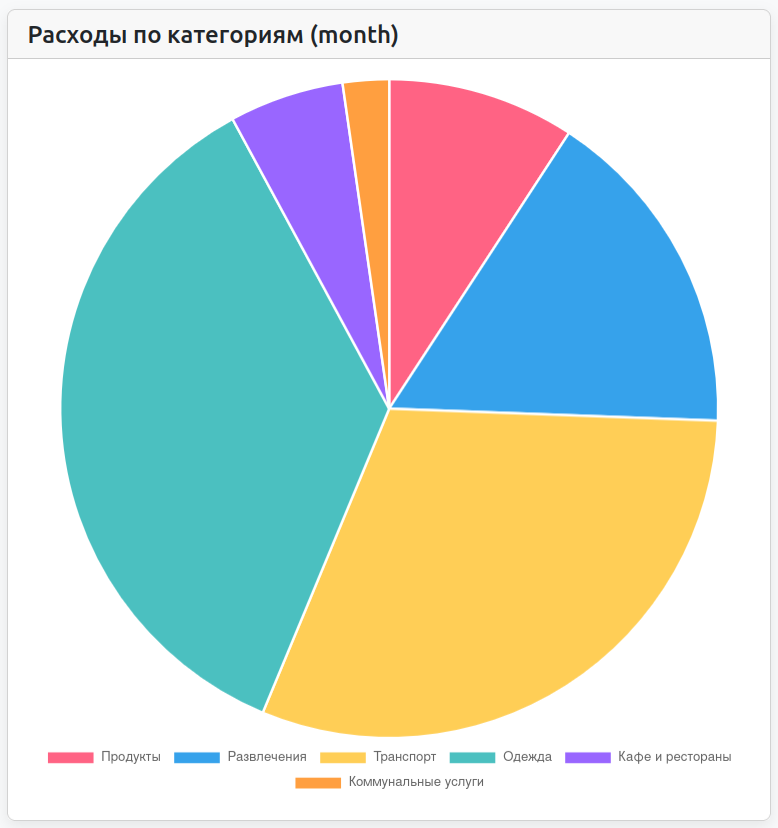
\includegraphics[width=0.7\textwidth]{images/pie_chart.png}
    \caption{Круговая диаграмма расходов по категориям}
    \label{fig:pie_chart}
\end{figure}

\textbf{Столбчатая диаграмма динамики баланса}

Показывает изменение баланса по дням выбранного периода. Данные передаются через переменные \texttt{chart\_labels} (метки дат) и \texttt{chart\_balance\_data} (значения баланса). Для владельца диаграмма имеет цветовое кодирование: зелёные столбцы для дней с положительным балансом, красные — для отрицательных, серые — для будущих дней. Диаграмма строится с типом \texttt{bar}.

\begin{figure}[H]
    \centering
    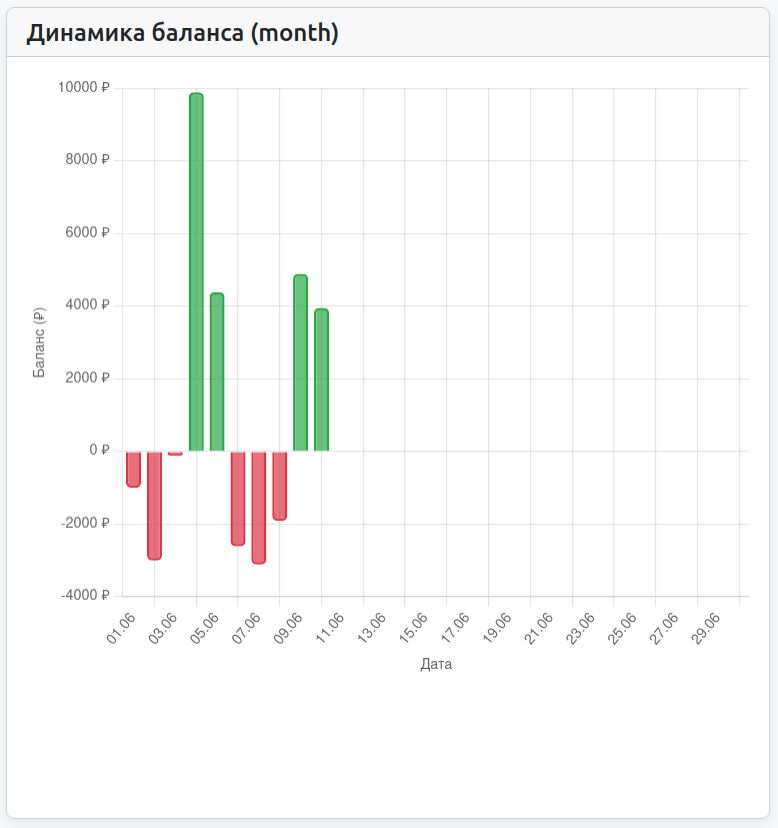
\includegraphics[width=0.7\textwidth]{images/bar_chart.png}
    \caption{Столбчатая диаграмма динамики баланса}
    \label{fig:bar_chart}
\end{figure}

\textbf{Сводная таблица по участникам}

На дашборде владельца реализована таблица с агрегированными данными по каждому участнику семьи: доходы, расходы, баланс. Для каждого участника предусмотрена кнопка «Дашборд», открывающая детальную статистику участника.

\begin{figure}[H]
    \centering
    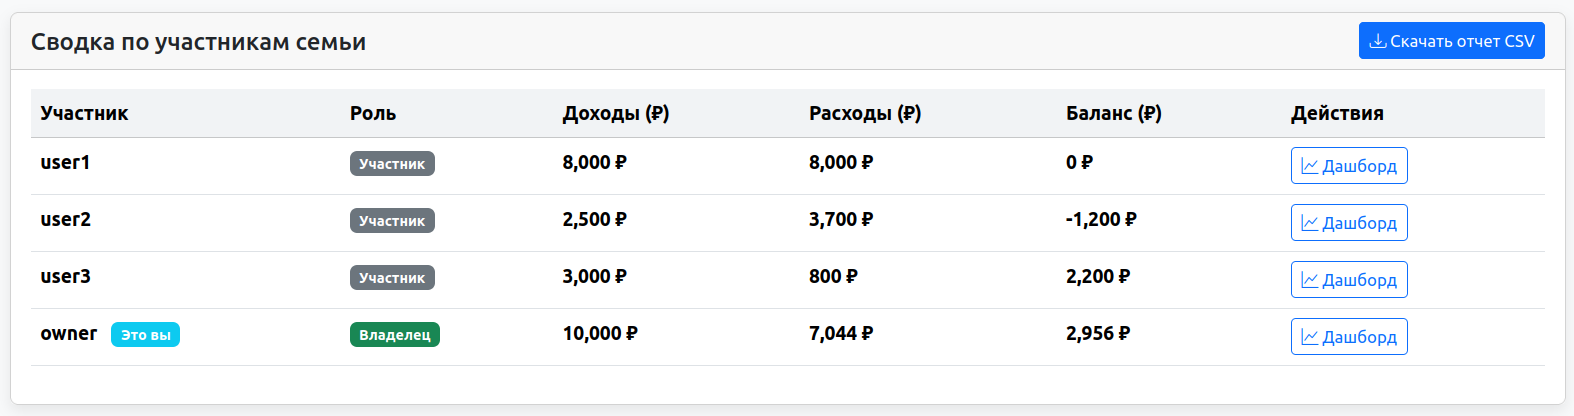
\includegraphics[width=0.9\textwidth]{images/members_table.png}
    \caption{Сводная таблица по участникам семьи}
    \label{fig:members_table}
\end{figure}

Все диаграммы автоматически перестраиваются при изменении периода через параметр URL \texttt{?period=}.


% Заключение
\section*{Заключение}
\addcontentsline{toc}{section}{Заключение}

В ходе выполнения курсового проекта было разработано веб-приложение для ведения семейного бюджета \texttt{MoneyManage}. Приложение позволяет семьям совместно контролировать доходы и расходы, устанавливать бюджеты для участников, загружать чеки и получать наглядную статистику.

В результате выполнения работы были решены все поставленные задачи:

\begin{enumerate}
    \item Проведён анализ существующих программных продуктов (Дзен-мани, CoinKeeper, Money Lover), выявивший их недостатки: платные премиум-функции, слабая поддержка совместной работы, отсутствие полноценных веб-версий. Обоснован выбор технологического стека: Python + Flask, PostgreSQL, Bootstrap 5, Chart.js.
    
    \item Определены требования целевой аудитории (семьи с совместным бюджетом) и спроектирована функциональность приложения, включая диаграммы вариантов использования и User Story.
    
    \item Разработана модель данных, включающая 8 сущностей (\texttt{Family}, \texttt{User}, \texttt{Category}, \texttt{Transaction}, \texttt{Receipt}, \texttt{CategoryLimit}, \texttt{UserBudget}, \texttt{DashboardStats}), построена ER-диаграмма.
    
    \item Созданы макеты страниц (wireframes) для всех категорий пользователей: администратора, владельца семьи и участника.
    
    \item Реализована система аутентификации и авторизации с тремя ролями (\texttt{admin}, \texttt{owner}, \texttt{member}) с использованием \texttt{Flask-Login} и \texttt{bcrypt}. При регистрации владельца автоматически создаются категории по умолчанию.
    
    \item Разработан CRUD-интерфейс для транзакций, категорий и участников. Реализованы фильтрация транзакций по дате и поиску, установка лимитов на категории и персональных бюджетов.
    
    \item Реализованы механизмы загрузки чеков (изображения, PDF) с сохранением на сервере и хранением пути в БД. Добавлен экспорт отчётов в формате CSV.
    
    \item Реализована система визуализации: круговая диаграмма расходов по категориям и столбчатая диаграмма динамики баланса (Chart.js). Для оптимизации производительности используется кэширование ежедневных балансов в модели \texttt{DashboardStats}.
    
    \item Проведено тестирование приложения, код размещён в репозитории GitHub: \url{https://github.com/userownmaa/web_coursework_Momina_241-327}. Оформлена отчётная документация.
\end{enumerate}

Разработанное приложение представляет собой полноценный программный продукт, готовый к развёртыванию на хостинге. Дальнейшее развитие проекта может включать: добавление мобильной версии, интеграцию с банковскими API для автоматического импорта транзакций, расширенную аналитику с прогнозированием расходов, а также улучшение системы уведомлений о превышении лимитов.


% Список литературы
\bibliographystyle{ugost2003} % ГОСТ 7.1-2003
\bibliography{refs}

% Приложения (при необходимости)
% \include{appendix}

\end{document}
